% Document class options:
% =======================
%
% serif: Sets the body font to be serif.
%
% twocolumn: Sets the body text in two - column layout.
%
% Fill in the type of article here.
% empirical
  % reflection
  % meta
  % rga
  % editorial
  %
% Using other bibliography styles:
% =======================
% authordate = APA
  % number =[1]
  %
    \documentclass[twocolumn, serif, rga, authordate]{jote-article}


  %%% Add the bibliography, make sure it's in the same directory
\addbibresource{schwalbe.bib}

%%% Add additional packages here if required.Usually not needed, except when doing things with figures and tables, god help you then

  % This package is for generating Lorem Ipsum, usage: \lipsum[X] where X is the Xth paragraph of lorem ipsum.OR use[1 - 5] to generate the first five, etc.

\usepackage{gensymb}
\usepackage{graphicx}
\usepackage[export]{adjustbox}% http://ctan.org/pkg/adjustbox


%%% TODO: Make this a 1 - 5 option scale to reduce the chance of mistyping

  % Enter the title, in Title Case Please
    % Try to keep it under 3 lines
\title{Communication Circuits and Inequalities of Health: A Case of Greenlanders in Denmark}

% List abbreviations here, if any.Please note that it is preferred that abbreviations be defined at the first instance they appear in the text, rather than creating an abbreviations list.
%\abbrevs{
%  ABC, a black cat; DEF, doesn't ever fret; GHI, goes home immediately.}

    % Include full author names and degrees, when required by the journal.
% Use the \authfn to add symbols for additional footnotes and present addresses, if any.Usually start with 1 for notes about author contributions; then continuing with 2 etc if any author has a different present address.
% Format: \author[1, 2]{FirstName LastName} \author[2]{...}
  \author[1]{Daria Schwalbe}

    % Fill it in again for the PDF metadata.Lame workaround but it works
      % Format: \authorone{...} \authortwo{...}
  \authorone{Daria Schwalbe}

    % List the contribution effort here, they will be listed at the end of the page
      % List the acknowledgments.If there is no companion piece, this is listed below the author info
        %\acknowledgments{Author Two would like to thank Author One for doing all the work while they could slack off.}
% List possible conflict of interest.Will default to saying no conflict exists.
%\interests{Author One was paid for by Big Failed Experiment}
% List funding
    %\funding{}
% Include full affiliation details for all authors
\affil[1]{University of Southern Denmark, SDU · Department of Language and Communication}

    % List the correspondence email of the main correspondent
  \corraddress{corraddressmarker}
  \corremail{\href{dschwalbe@sdu.sk}{dschwalbe@sdu.sk}}

% Optionally list the present address of one of the authors
    %\presentadd[\authfn{2}]{Department, Institution, City, State or Province, Postal Code, Country}

% Fill in the DOI of the paper

    % Always starts with '10.36850/' and is suffixed with one of the following plus a number
      % e  : empirical
        % r  : reflection
          % mr : meta - research
            % rga: rejected grant application
              % ed : editorial
  \paperdoi{10.36850/rga4}

% Include the name of the author that should appear in the running header
  \runningauthor{Schwalbe}

% The name of the Journal
  \jname{Journal of Trial and Error}

% The year that the article is published
  \jyear{2021}

% The Volume Number
    %\jvolume{Fall}

% The website that's listed in the bottom right
  \jwebsite{
    https://www.jtrialerror.com}

%%% Only \paperpublished is necessary, any combination of the other two is possible

      % When the paper was received
        % Format: 1 January, 1900
    \paperreceived{}
% When the paper was accepted
      % Format: 1 January, 1900
    \paperaccepted{}
% When the paper will be published
      % Format: 1 January, 1900
    \paperpublished{24 December, 2021}
% When the paper is published but in YYYY - MM - DD format, for the crossmark button
    \paperpublisheddate{2021-12-22}

% The pages of the article, comment out if rolling article
      %\jpages{1 - 12}
% Link to the logo, might be redundant
    \jlogo{media/jote_logo_full.png}

% Fill something here if this is a rolling / online first article, will make ROLLING ARTICLE show up on the first page
    \rolling{}

% Sets the paragraph skip to be zero, this should be in the CLS
    \setlength{\parskip}{0pt}

    \acknowledgments{\emph{The author would like to express her gratitude to both Naja Blytmann Trondhjem, associate professor, University of Copenhagen, for her collaboration on the research proposal, and to \href{https://tors.ku.dk/ansatte/?pure=da\%2Fpersons\%2Fcharlott-hoffmann-jensen(a4b7c387-1e34-44c0-b70a-cbb7ea85c882).html}{Charlott Hoffman, chief consultant at the Department of Cross-Cultural Regional Studies, Copenhagen University}), who provided indispensable help with the revision of the manuscript and budget development. }}
%%% Companion Piece

      % Reflection and Empirical articles have each other as companion pieces.Add the DOI, Title, and Abstract of the respective Companion piece here

        %%% Abstract

        % These two set the height and width of the abstract.There's no solution to do this automatically at the moment so fiddle with these a bit. height-width should be 5mm, and ranges between 50-100 are realistic
          % Higher number means skinnier abstract
    \heightabstract{55mm}
    \widthaffil{50mm}
    %\rgainfo{Independent Research Fund Denmark -- 2018}
% Enter something here in order for the abstract to disappear.Be sure to also delete the abstract
    \noabstract{}
% Fill in the keywords that will appear in the abstract, max 7
    \keywordsabstract{language, health, communication, equality, Greenlanders in Denmark}

%%%%%%%%%%%%%%%%%%%%%%%%%%%%%%%%%%%%%%%%%%%%%%%%%%%
% Document Starts
      %%%%%%%%%%%%%%%%%%%%%%%%%%%%%%%%%%%%%%%%%%%%%%%%%%%

    \begin{document}
%%% This starts the frontmatter, which includes everything that's on the front page execpt the text of the article
    \begin{frontmatter}
    \maketitle
      % Type your abstract between these things.Max 250 words.Be sure to include the \noindent, looks bad otherwise
    \begin{abstract}

Discourses surrounding migration and integration often see language, and in particular the knowledge of the native language, as a crucial barrier to minorities' access to healthcare and welfare benefits, equal healthcare treatment, social integration, and psychological wellbeing.
Using methods of ethnographic and interactional sociolinguistic and conversational analysis our project investigates how healthcare and welfare professionals and Greenlandic patients define, interpret and manage communication and language inequalities in face-to-face encounters. What are the practical, cognitive, psychological and social consequences of ``miscommunication'' for the Danish Greenlanders? We examine four distinct aspects of communication: conversational strategies, non-verbal behavior, linguistic insecurity, and attitudes.
Our aim is to understand the entire communicative circuit (i.e. channels by which information is transmitted), developing on our idea of
``affective language economies of health''.
    \end{abstract}
    \end{frontmatter}




\section*{Research proposal}



\subsection*{General Information}



\subsubsection*{Institution of employment at time of application}


Copenhagen Business School, Department of Management, Society and Communication


\subsubsection*{Prospective host institution}


University of Copenhagen, Department of Cross-Cultural and Regional Studies


\subsubsection*{Main field}


Intercultural communication, health studies


\subsubsection*{Other fields}


Anthropology/linguistics


\subsubsection*{Length requirement}


7 pages, 22.000 characters, including tables, but excluding bibliography


\subsection*{Description of the proposed research}


Language, and in particular knowledge of the Danish language, is often seen as a crucial barrier to equal healthcare treatment and to minorities' access to Danish healthcare and welfare benefits.

Sharing the national and international ambition to achieve more equity in healthcare and welfare system, this research project investigates the role language and non-verbal behaviour play, when Greenlanders move to Denmark and encounter the Danish healthcare and welfare professionals
(SVPs), and where this poses a potential communication barrier. Our aim is to examine the entire communicative circuit (i.e. channels by which information is transmitted), providing new empirical knowledge and theoretical insights into the emerging field of study of language and health.


\subsubsection*{Aim and objectives}



\paragraph{The main objectives are}

\begin{itemize}
\item Empirically, we seek to elucidate how language ideologies (i.e. sets of beliefs and ideas about language articulated by users), continuously reproduced in institutionalized practices, and nonverbal behaviour may lead to a feeling of miscommunication and injustice among the Greenlandic patients, cause cognitive blocking, emotional stress, self-exclusion and feelings of injustice among them. It will provide new original knowledge about the context-specific tendencies and potentials that occur when people with distinct social, health, psychological, and communicative ``challenges'' meet the Danish SVPs, and add new knowledge on values and behaviour (verbal and non-verbal) of Greenlanders in Denmark.

\item Theoretically, this study seeks to expand the field of study of language and health by bridging health studies with intercultural communication theories, linguistics, and emotional theories under what we call ``affective language economies of health''.

\item Together with public sector partners and professional universities we seek to develop a method through which identified by participants barriers may be overcome or reduced in the everyday practice of SVPs in their encounters with patients, who have a different first language.

        \end{itemize}

\paragraph{Research questions}

The objectives will be pursued by focusing on the following research questions:

\emph{To what extend does language (linguistic proficiencies and ideologies) and non-verbal behaviour influence communication in clinical encounters and welfare in Denmark? What are the practical, societal, health and psychological consequences of potential miscommunication for the patients?}


\paragraph{Empirical focus: the Danish greenlanders}


In the recent years, there has been an increasing focus in the Danish media and among the Danish researchers and policy makers on social integration and inclusion of ethnic minorities (migrants, refugees and asylum seekers) from countries outside of Nordic countries, EU and North America. Greenlanders, on the other hand, have been ``overlooked'' in the Danish context.

As of today, there are 16.370 Greenlanders in Denmark. This number is constantly growing.

Another thousand come to Denmark each year to receive medical treatment.
Yet, because Greenlanders are Danish citizens they are not offered the same integration aid as refugees and immigrants when they visit for health treatment or move to Denmark. Not only does this ``lack of integration effort'' contrasts Canada and the US attempts to accommodate indigenous minorities' cultural and linguistic needs in recognition of Indigenous rights, but it is also ``a form of misunderstood equality that you will treat the Greenlanders as Danish nationals and give them the same rights'' (\pdftooltip{{\color{tip}Toft,}}{V, K. P. (Ed.). (2002). Regimes of Language: Ideologies, Polities, and Identities.} \citeyear{Toft2018}).

Indeed, although about 80\% of Greenlanders manage well, and the majority are well integrated into Danish society, there is still a great distance between Denmark and Greenland, geographically, culturally, and linguistically. Similar to refugees, many Greenlanders who arrive in Denmark have experienced social problems at home and/or have been traumatised (\pdftooltip{{\color{tip}Laage-Petersen,}}{Maintenance and Loss. (n.d.). Sibirica, 14(3), 1–27.} \citeyear{laage-petersen2015}). Many lack a regular income, feel socially isolated and/or anxious living on their own in Denmark
(\pdftooltip{{\color{tip}Socialministeriet,}}{Silverstein, M. (1979). Language Structure and Linguistic Ideology. In R. Clyne, W. Hanks, \& C. Hofbauer (Eds.), The elements: parasession on linguistic units and levels (pp. 193–247). Chicago Linguistic Society.} \citeyear{Socialministeriet2003}). They too experience prejudice and discrimination when encountering the Danish public authorities and healthcare. According to recent sociological research language (``poor Danish language skills''), negative representations and stigmatization of Greenlanders, and lack of knowledge of rights and appeal regulation procedures are among the major challengers (\pdftooltip{{\color{tip}Laage-Petersen,}}{Maintenance and Loss. (n.d.). Sibirica, 14(3), 1–27.} \citeyear{laage-petersen2015}; \pdftooltip{{\color{tip}Togeby}}{Wierzbicka, A. (2014). Imprisoned in English. The Hazards of English as a Default Language. Oxford University Press.}, \citeyear{Togeby2004}).

According to Heidi Conradsen, project manager at Oqqumut, Activation Center for Greenlanders in Esbjerg Municipality, welfare professionals often experience ``significant cultural differences'' with regard to conversation style, humility, and a general lack of societal understanding (personal communication). In the White Paper on "socially disadvantaged Greenlanders", The Danish Ministry of Social Affairs points out that Danish welfare and healthcare professionals need concrete help in order to recognize Greenlanders special needs and address the challenges, because Greenlanders are often met with prejudice, negative and stigmatizing expectations, which may become ``a self-fulfilling prophesy'' (Socialministeriet 2003 s.21). Nonetheless, healthcare professionals and social workers are not offered any specific training.

Our project addresses some of these critical issues by investigating situated practices (what is actually going on in conversations between Greenlanders and SVP's) and experiences of the mentioned above characteristics and of clinical encounters of a selected group of Greenlanders. In the analysis, we focus on four distinct aspects of communication: language proficiencies, conversational styles, societal attitudes, and non-verbal behaviour.


\paragraph{Theoretical approach}


Previously, researchers have focused mainly on social inequality as an effect of negative biases (social stereotypes and prejudiced attitudes)
against Greenlanders in Denmark, measuring reported behaviours and attitudes (\pdftooltip{{\color{tip}Togeby,}}{Wierzbicka, A. (2014). Imprisoned in English. The Hazards of English as a Default Language. Oxford University Press.} \citeyear{Togeby2004}; \pdftooltip{{\color{tip}Laage-Petersen}}{Maintenance and Loss. (n.d.). Sibirica, 14(3), 1–27.}, \citeyear{laage-petersen2015}).
These studies do not look at what is actually going on during the encounters, nor do they address the role language (linguistic competences and ideologies) actually plays in the construction of these biases.

Yet, as a series of linguistic anthropological studies have shown, languages is anything but neutral. Language is not only crucial for immigrants' political and social participation, and individual's ability to communicate with the national authorities (\pdftooltip{{\color{tip}Togeby,}}{Wierzbicka, A. (2014). Imprisoned in English. The Hazards of English as a Default Language. Oxford University Press.} \citeyear{Togeby2004}), but it is also a prerequisite of economic and psychological wellbeing in a foreign country (\pdftooltip{{\color{tip}Chiswick \& Miller,}}{Briggs, C. L. (2005). Communicability, Racial Discourse, and Disease. Annual Review Of.} \citeyear{Chiswick1995};
\pdftooltip{{\color{tip}Ting-Toomey}}{Toft, S. B. (2018). Grønlændere lades i stikken af deres danske statsborgerskab”. Information.}, \citeyear{ting-toomey2011}). Because ways of speaking often become a way through which people are identified and judged, and through which legitimacies and illegitimacy, inclusion and exclusion, and group identities are symbolized (\pdftooltip{{\color{tip}Aikhenvald,}}{Aikhenvald, A. (2002). Language Contact in Amazonia. Oxford University Press.} \citeyear{Aikhenvald2002}; \pdftooltip{{\color{tip}Blackledge}}{Basso, K. H. (1970). To Give up on Words: Silence in Western Apache Culture. Southwestern.}, \citeyear{Blackledge2002}; \pdftooltip{{\color{tip}Piller}}{O’Neil, J. D., Kaufert, J. M., \& Koolage, W. W. (1989). Taking a medical history in a cross-cultural context: the role of the medical interpreter. Manitoba Medicine, 59(3), 101–104.}, \citeyear{Piller2016}; \pdftooltip{\color{tip}Schwalbe}{Schwalbe, D. M. (2015). Language ideologies at work: Economies of yupik
language maintenance and loss.} \citeyear{Schwalbe2015}; \pdftooltip{{\color{tip}Woolard}}{(N.d.-b). Humanities, University of Copenahgen.}, \citeyear{Woolard1998}), a lack of necessary language skills may lead to negative categorization, exclusion, and ethnic segregation (\pdftooltip{{\color{tip}Ting-Toomey,}}{Toft, S. B. (2018). Grønlændere lades i stikken af deres danske statsborgerskab”. Information.} \citeyear{ting-toomey2011}).
Moreover, negative attitudes towards certain ways of speaking may cause a feeling of insecurity, unworthiness, and low self-esteem. This may block cognitive ability of the exposed, leading to lack of motivation, participation refusal and self-exclusion (\pdftooltip{{\color{tip}Collier \& Thomas,}}{Ting-Toomey, S. (2011). Communicating across cultures. The Guilford Press.} \citeyear{Collier2001}).

In this research project, we shall focus on how imaginations of language
(and ``justice'') affect speakers' perceptions of each other and their sense of belonging. Since non-verbal communication affects individual's sense of belonging -- it is through non-verbal cues that groups'
identities and relations are symbolized (studies have in fact claimed that between 65 and 80 \% of the message is communicated non-verbally, cf. \pdftooltip{{\color{tip}Hall}}{Hall, E. T. (1998). The power of hidden differences. In M. J. Bennett (Ed.), Basic concepts of intercultural communication: Selected readings (pp. 53–67). Intercultural Press. Pp.} \citeyear{Hall1959}; \pdftooltip{{\color{tip}Ting-Toomey}}{Toft, S. B. (2018). Grønlændere lades i stikken af deres danske statsborgerskab”. Information.}, \citeyear{ting-toomey2011}) -- we also attend the non-verbal
``rules'' of behaviour that at play when Greenlandic patients meet the Danish SVPs.


\paragraph{Methods ethnographic and linguistic}


Our focus is on situated interaction, i.e. what people actually do and say or not say, how they say it, when and under what circumstances. We are interested in both the linguistic (language proficiencies, conversational strategies, styles of communication, turn-taking) and the non-verbal (body positioning, gestures, facial expressions, eye contact, smile, tone of voice, intonation, irony, silence and restrain) aspects of communication. We have identified 5 priority sub-topics: (1) turn-taking (2) silence (3) trust and restrain
(4) linguistic insecurity (5) directness vs. indirectness.

We draw on methods and findings of interactional (\pdftooltip{{\color{tip}Schegloff,}}{Schegloff, E.A. (1991). Conversation Analysis and Socially Shared Cognition. In L. Resnick, J. M. Levine, \& S. D. Teasley (Eds.), Perspectives on Socially Shared Cognition. American Psychological Association.} \citeyear{Schegloff1990};
Gumperz 1982) and ethnographic (\pdftooltip{{\color{tip}Hymes,}}{Hong, Y. Y., Morris, M. W., Chiu, C. Y., \& Benet-Martinez, V. (2000). Multicultural minds: A dynamic constructivist approach to culture and cognition. American Psychologist, 55(7), 709–720.} \citeyear{Hymes1962};\pdftooltip{  }{Hymes, D. (1962). The Ethnography of Speaking. In T. Gladwin \& W. C. Sturtevant (Eds.), Anthropology and Human Behavior. The Anthropological Society of Washington. Pp.:13–53.}\citeyear{Hymes1964}; \pdftooltip{{\color{tip}Basso}}{Alexander, J. C. (n.d.). eds.): The Micro-Macro Link. University of California Press.}, \citeyear{Basso1970}) sociolingusitics, cultural studies (\pdftooltip{{\color{tip}Goffman,}}{Forlag, R. (n.d.).} \citeyear{Goffman1974};\pdftooltip{  }{Alexander, J. C. (n.d.). eds.): The Micro-Macro Link. University of California Press.) sociolingusitics, cultural studies (\pdftooltip{{\color{tip}Goffman,}}{Forlag, R. (n.d.).} \citeyear{Goffman1982}}\citeyear{Basso1970}) sociolingusitics, cultural studies (\pdftooltip{{\color{tip}Goffman,}}{Forlag, R. (n.d.).} \citeyear{Goffman1982}; \pdftooltip{{\color{tip}Hall}}{Goffman, E. (1982). Interaction Ritual: Essays on face-to-face behavior. Pantheon.}, \citeyear{Hall1997}Riggins 1997), and intercultural communication theory (\pdftooltip{{\color{tip}Hall,}}{Gumperz, J. J., \& Hymes, D. (Eds.). (1972). Directions in Sociolinguistics: The Ethnography of.} \citeyear{Hall1959}; \pdftooltip{{\color{tip}Johnstone}}{intercultural communication: Selected readings (pp. 53–67). (n.d.). Intercultural Press. Pp.}, \citeyear{Johnstone1989}, \pdftooltip{{\color{tip}Meyer }}{Meyer, I. (2014). The culture map. Breaking through the invisible boundaries
of global business. Public Affairs.} \citeyear{Meyer2014}). The analysis builds on the work of \pdftooltip{{\color{tip}Aagaard}}{Aagaard, T. (2014). Hverdagsliv med sygdom : patienters kulturelle perspektiver på sundhedspraksis i Grønland (p. 263) [Ph.d. thesis,]. Institut for Sygepleje og Sundhedsvidenskab.} (\citeyear{Aagaard2014}) on patients' cultural perspective on healthcare in Greenland, \pdftooltip{{\color{tip}Curtis}}{Curtis, T. (2001). Kommunikation mellem læge og partient i Grønland – en
kvalitative undersøgelse af interaktionen mellem parterne i den
tolkende konsultationssamtale} (\citeyear{Curtis2001}) and \pdftooltip{{\color{tip}Kaufert \& O'Neil}}{Kaufert, J. M., & Putsch, R. W. (1997). Communication through interpreters in healthcare: ethical dilemmas arising from differences in class, culture, language, and power. Journal Clinical Ethics, 8(1), 71–87.} (\citeyear{Kaufertt1998};\pdftooltip{{\color{tip}Goffman}}{Goffman, E. (1982). Interaction Ritual: Essays on face-to-face behavior. Pantheon.Riggins 1997}\citeyear{Goffman1982}), and intercultural communication theory (\pdftooltip{{\color{tip}Hall,}}{Gumperz, J. J., \& Hymes, D. (Eds.). (1972). Directions in Sociolinguistics: The Ethnography of.} \citeyear{Hall1959}; \pdftooltip{{\color{tip}Johnstone}}{intercultural communication: Selected readings (pp. 53–67). (n.d.). Intercultural Press. Pp.}, \citeyear{Johnstone1989}; \pdftooltip{{\color{tip}Meyer}}{Meyer, I. (2014). The culture map. Breaking through the invisible boundaries
of global business. Public Affairs.}, \citeyear{Meyer2014}). The analysis builds on the work of \pdftooltip{{\color{tip}Aagaard}}{Aagaard, T. (2014). Hverdagsliv med sygdom : patienters kulturelle perspektiver på sundhedspraksis i Grønland (p. 263) [Ph.d. thesis,]. Institut for Sygepleje og Sundhedsvidenskab.} (\citeyear{Aagaard2014}) on patients' cultural perspective on healthcare in Greenland, \pdftooltip{{\color{tip}Curtis}}{Brussels/Artistic Rights Society (ARC. (n.d.).} (\citeyear{Curtis2001}) and \pdftooltip{{\color{tip}Kaufert \& O'Neil}}{Johnstone, B. (1989). Linguistic strategies and cultural styles for persuasive discourse. In S. Ting-Toomey \& F. Korzenny (Eds.), Language, communication, and culture: Current directions (pp. 139–156).} (\citeyear{Kaufert1998, Hall1997, Riggins1997}), and intercultural communication theory (\pdftooltip{{\color{tip}Hall,}}{Gumperz, J. J., \& Hymes, D. (Eds.). (1972). Directions in Sociolinguistics: The Ethnography of.} \citeyear{Hall1959}; \pdftooltip{{\color{tip}Johnstone}}{intercultural communication: Selected readings (pp. 53–67). (n.d.). Intercultural Press. Pp.}, \citeyear{Johnstone1989}Meyer 2014). The analysis builds on the work of \pdftooltip{{\color{tip}Aagaard}}{Aagaard, T. (2014). Hverdagsliv med sygdom : patienters kulturelle perspektiver på sundhedspraksis i Grønland (p. 263) [Ph.d. thesis,]. Institut for Sygepleje og Sundhedsvidenskab.} (\citeyear{Aagaard2014}) on patients' cultural perspective on healthcare in Greenland, \pdftooltip{{\color{tip}Curtis}}{Brussels/Artistic Rights Society (ARC. (n.d.).} (\citeyear{Curtis2001}) and \pdftooltip{{\color{tip}Kaufert \& O'Neil}}{Kaufert, J. M., Putsch, R. W., & Lavallee, M. (1998). Experience of aboriginal health interpreters in mediation of conflicting values in end-of-life decision-making. International Journal of Circumpolar Health, 57 Suppl 1, 43–8} (\citeyear{Kaufert1998}) work on the role of interpreters in clinical encounters. When developing the idea of `language economies', i.e.
systems of demand and supply displayed in group's dynamics, we draw on \pdftooltip{{\color{tip}Bourdieu}}{Blackledge, A., \& Pavlenko, A. (2002). Introduction. Multilingua, 21(2–3), 121–140.} (\citeyear{Bourdieu1991}) notion of linguistic capital and on \pdftooltip{{\color{tip}Briggs}}{Books. (1982).} (\citeyear{Briggs2005}) idea of communicability, i.e. ``the productive relation between discursive ideologies or practices and social relations'' as a way of understanding how diversity is managed within a society.


\subsubsection*{Research plan}


In order to achieve our academic, societal, and practical goals, the research will be organised in three phases: (P1) ethical approvals, research planning, and data-collection and analysis; (P2) comparative data-analysis and data-collection (P3) a practice-development and dissemination phase. P1 will be divided into four work-packages:

\begin{itemize}
\item WP1: \textbf{Greenlander's encounters with the danish healthcare professionals}


\item WP2:
\textbf{Greenlanders encounters with welfare professionals}


\item WP3:
\textbf{Greenlandic way of talking a comparative perspective}


\item WP4:
\textbf{Practice development}
        \end{itemize}


\paragraph{\emph{WP 1: Greenlanders's encounters with the Danish Healthcare professionals} (University of Copenhagen (UCPH) \& Copenhagen University Hospital)}

This research will be conducted by principal investigator Daria Schwalbe
(DS), in collaboration with Unit for Greenlandic Coordination, Copenhagen University Hospital. Following methods of interactional linguistics (\pdftooltip{{\color{tip}Gumperz,}}{Gumperz, J. J., \& Hymes, D. (Eds.). (1972). Directions in Sociolinguistics: The Ethnography of Communication (pp. 407–434). Holt, Rinehart. (Original work published 1964) Original work published 1964} \citeyear{Gumperz1972}) and conversational analysis (\pdftooltip{{\color{tip}Schegloff,}}{Schegloff, E.A. (1991). Conversation Analysis and Socially Shared Cognition. In L. Resnick, J. M. Levine, \& S. D. Teasley (Eds.), Perspectives on Socially Shared Cognition. American Psychological Association.} \citeyear{Schegloff1990};\pdftooltip{  }{Gumperz, J. J., \& Hymes, D. (Eds.). (1972). Directions in Sociolinguistics: The Ethnography of Communication (pp. 407–434). Holt, Rinehart. (Original work published 1964) Original work published 1964}\citeyear{Gumperz1972}) and conversational analysis (\pdftooltip{{\color{tip}Schegloff,}}{Schegloff, E.A. (1991). Conversation Analysis and Socially Shared Cognition. In L. Resnick, J. M. Levine, \& S. D. Teasley (Eds.), Perspectives on Socially Shared Cognition. American Psychological Association.} \citeyear{Schegloff1991}; \pdftooltip{{\color{tip}Gumperz}}{Gumperz, J. J., & Hymes, D. (Eds.). (1972). Directions in Sociolinguistics: The Ethnography of Communication (pp. 407–434). Holt, Rinehart. (Original work published 1964) Original work published 1964}, \citeyear{Gumperz1972}) and conversational analysis (\pdftooltip{{\color{tip}Schegloff,}}{Schegloff, E.A. (1991). Conversation Analysis and Socially Shared Cognition. In L. Resnick, J. M. Levine, \& S. D. Teasley (Eds.), Perspectives on Socially Shared Cognition. American Psychological Association.} \citeyear{Schegloff1991}), we will use a three-fold ethnographic data-collection method: 1)
Method of observation will be used when collecting data on clinical encounters (scheduled appointments and patient-conversations) between the Danish health care professionals at the Copenhagen University Hospital and the Danish-speaking Greenlanders. To access different types of clinical care pathways and patient-conversations, data-collection will be carried out at three departments at the Copenhagen University Hospital: cardiology, thoracic surgery, and haematology at Copenhagen University Hospital (\emph{Rigshospitalet}), and spinal cord surgery at Glostrup Hospital. The predominant analytical focus in this type of data collection is on communicative strategies and styles (said and unsaid in a conversation, directness, indirectness, silence and restrain), and non-verbal behaviour as communicative barriers. To investigate both the verbal and non-verbal aspects of communication, clinical encounters will be video recorded. 2) Method of participant-observations will be used to observe patient rounds, nursing encounters, educational group sessions
(at Glostrup Hospital) and daily routines of the patients; 3) Methods of semi-structured interviews with patients and healthcare professionals will be conducted to understand how the participants experience and interpret clinical encounters, language proficiencies, and non-verbal behaviour (\pdftooltip{{\color{tip}Spradley,}}{Steensig, J. (2011). Turn-taking in conversation. In G. Andersen \& K. Aijmer (Eds.), Pragmatics of Society. Mouton de Gruyter.} \citeyear{Spradley1997}).

  \paragraph{\emph{WP 2: Greenlanders' encounters with welfare professionals} (UCPH \& The House of Greenlanders in Copenhagen \& Oqqumut, Esbjerg Municipality)}

In collaboration with the House of Greenlanders, we will obtain access to a group of Greenlanders who have migrated to Denmark within the past 10 years, including the newly arrived Greenlanders and those who have lived here for a substantial time period and who have had experiences with the Danish healthcare and welfare sectors. Comparing experiences of newcomers with those Greenlanders who have been already accommodated to the Danish society will allow us to see whether the tendencies are similar between the groups, enabling us to determine how their linguistic and communicative proficiencies (and experiences) change over time. This will allow us to document long-term integration processes. To get access to necessary segment of informants, we use our already established contact to the House of Greenlanders and their network.
Compared to healthcare, communication with welfare professionals in a Greenlandic context is often linked to negative emotions, such us shame and distrust. We are thus particularly interested in exploring how emotional economies (``trust'', ``shame'' and ``restrain''), ``silence''
and ``directness'' may affect the encounter, and how these dynamics are different from clinical encounters. The research will use similar to WP1 methodology (video recordings, participant-observation and semi-structured interviews). To validate our data, we will conduct 6 focus group interviews with our Greenlandic participants (6-8 people each) with the help of a research assistant. These will be conducted at the House of Greenlanders in Copenhagen, recorded and transcribed.

\paragraph{\emph{WP 3: Greenlandic ways of talking (}ÙCPH \& The Greenlanders Patient Home in Copenhagen)}

To understand cultural and conversational differences that are at play, this part will focus on communication in Greenlandic, and more specifically on the turn-taking principle (\pdftooltip{{\color{tip}Tanen,}}{Tanen, D. (2012). Turn-taking and intercultural discourse and communication.
In C. B. Paulston, S. F. Kiesling, & E. S. Rangel (Eds.), The hand-
book of intercultural discourse and communication (pp. 135–157).
Blackwell.} \citeyear{Tanen2012}; \pdftooltip{{\color{tip}Steensig}}{SSteensig, J. (2011). Turn-taking in conversation. In G. Andersen & K. Aijmer
(Eds.), Pragmatics of society. Mouton de Gruyter.}, \citeyear{Steensig2011}) in Greenlandic. The data will be collected primarily at The Greenlanders'
Patient Home in Copenhagen, as well as include data from earlier investigations (\pdftooltip{{\color{tip}Trondhjem,}}{Woolard, K. (1998). Introduction: Language ideology as a field of inquiry. In B. Schieffelin, K. Woolard, \& P. Kroskrity (Eds.), Language Ideologies: Practice and Theory (pp. 3–47). Oxford University Press.} \citeyear{Trondhjem2008}). The data collected and investigated in this part of the project will be used as a comparative point to the main investigation of the intercultural communication between the Danish SVP and Greenlanders (WP1 and WP2). This part of the project will also shed light on turn-taking in Greenlandic, which has not been investigated before.

\paragraph{\emph{WP4: Practice development} (ÙCPH \& Copenhagen Business School)}
Together with CBS Teaching \& Learning Development and Support Unit and with public sector partners, DS and NT will develop strategies and educational materials
(case studies and educational videos) through which identified barriers may be overcome or reduced in the everyday practice of SVPs.

\subparagraph{Organisation of the research}

The project will be hosted at the Department of Cross-Cultural and Regional Studies, UCPH, and directed by Daria Schwalbe. Another key participant is Naja Trondhjem, associate professor, Greenlandic language specialist, UCPH. The core collaboration partners of the project are The Danish House of Greenlanders in Copenhagen and Copenhagen University Hospital. We use collaborative methodology (\pdftooltip{{\color{tip}Phillips,}}{Piller, I. (2016). Intercultural Communication - A Critical Introduction. Edinburgh University.} \citeyear{Phillips2018}), engaging our partners in the discussion of the production of knowledge. Project will be part of the Diversity and Difference Platform at CBS, which will allow us to bring organisational perspective into the research.

The project makes use of an Advisory Board (AB) and a Stakeholder Panel
(SP). \textbf{AB} consists of Associate Prof. Tenna Jensen, Center for Health Research in the Humanities, UCPH; Dr. Christina Larsen, senior advisor, Center for Peoples Health in Greenland, University of Southern Denmark; Prof. Alex Klinge, CBS; Prof. Louise Jane Phillips, Roskilde University; Prof. Josee Lavoie, Department of Community Health Sciences, University of Manitoba, Canada, and Associate Prof. Katie Cueva, Institute of Social and Economic Research University of Alaska, Anchorage, United States. The board will meet twice a year, during workshops or via videoconferences to discuss and identify productive theoretical questions and empirical findings. The Canadian and American researchers will be used as a testing ground for comparative interpretations and analyses.

\textbf{SP} includes Leise Johnsen, lead manager at The House of Greenlanders in Copenhagen; Pauline Albeck Thomsen, Greenlanders'
coordinator, Copenhagen University College; Aaja Chemnitz Larsen, The Danish Parliament, Inuit Ataqatigiit (IA); and Heidi Conradsen, Project manager at Oqqumut, Esbjerg Municipality. We are in a dialogue with Metropolian University College and Ilisimatusarfik. The Panel will meet twice a year to secure practical implementation and public outreach.

A full-time research assistant (RA) will be employed for a fixed term of two year to support data integration, international outreach, and practice development activities, including management of international symposium, revision and publication of symposium proceedings into an anthology.

\begin{figure*}
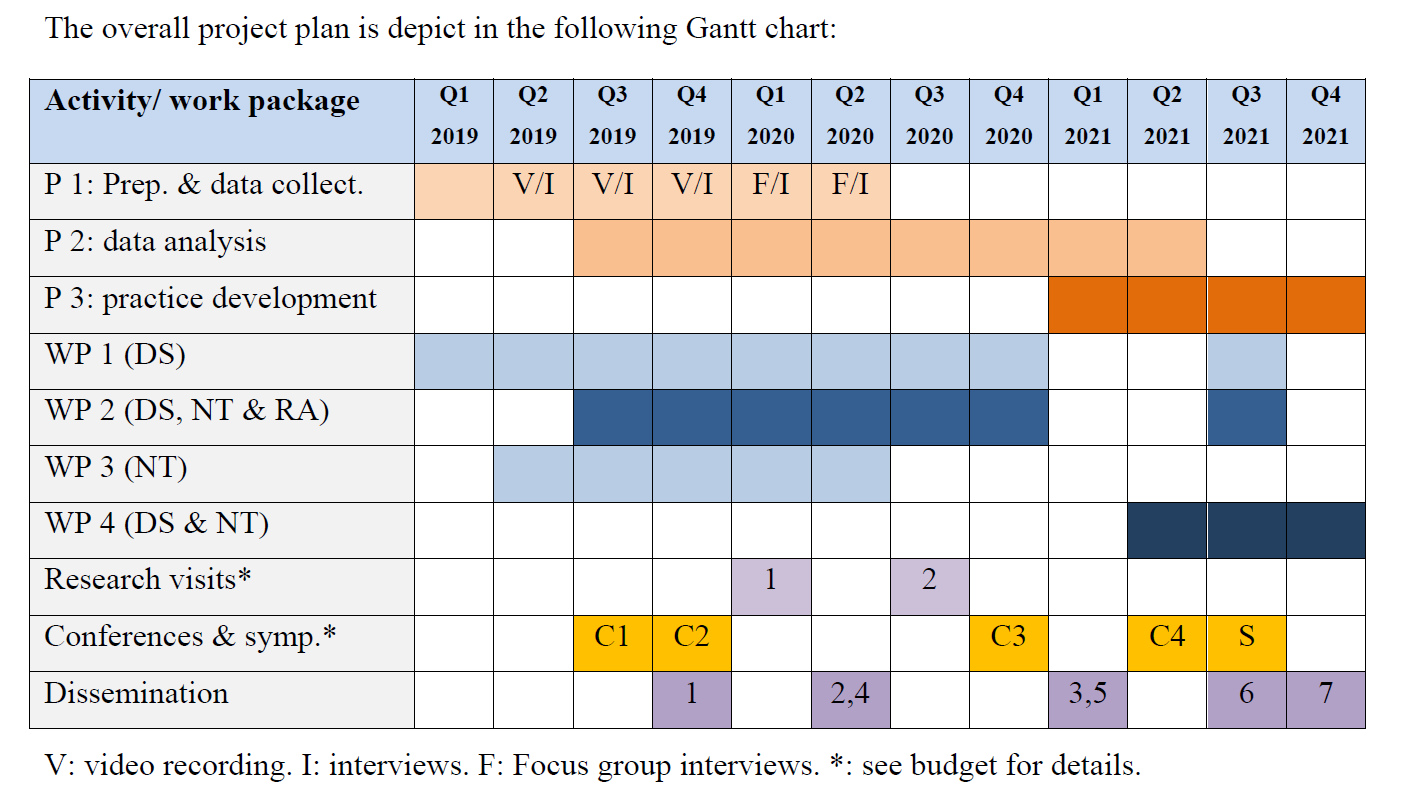
\includegraphics[width=\linewidth]{articles/RGAs/schwalbe/media/image1.png}
\caption{Overall project plan}

\end{figure*}

\subsection*{Knowledge Utilisation}



\subsubsection*{Potential}


\paragraph{Research}


Understanding how language and culture work in clinical encounters (and culture is communication, cf. Hall 1959), and how language
``difficulties'' and non-verbal behaviour may contribute to cultural biases, feeling of social injustice and exclusion is of extreme importance if we want to achieve a higher degree of participation and social inclusion, necessary to secure a more inclusive integration agenda and social cohesion in Denmark.


\subsubsection*{Implementation}



\paragraph{Research}


We will communicate our results at conferences and in Danish and international peer-reviewed publication channels, including
\emph{Inuit/Ethudes/Studies}, \emph{Linguistic Anthropology,} and
\emph{Journal of} \emph{Communication in Health Care}. The articles topics include: 1) ``Yes, no, I don't know'': cultural values in healthcare. 2) Imprisoned in Danish. 3) Trust, shame and restrain in a conversation 4) Silence and turn-taking in Greenlandic. 5) ``Keeping quite'': On the value of `quiet language'. 6) The negative effect of Danish directness. Proceedings of an international symposium on language and health in Copenhagen will be published in an anthology in English under the title ``Affective language economies of health'', with contribution from international researchers (7). Educational materials
(videos and case studies) for a broad pedagogical environment from university colleges to universities will be developed in the final stage of the project (WP4). We intend to establish Communication, Equality and Health Platform, and to offer interactive workshops for SVP's at the University Hospital and Municipalities across Denmark, and contribute with a feature article in a Danish and international newspaper.


\subsection*{Cost estimates}



\subsubsection*{Total budget requested}


4.284.188, excl. overheads


\subsubsection*{Intended starting date}


1.08.2019 (The project shall run for 3 $1/2$ years. Estimated end date is 31.01.2023)


\subsubsection*{Application for additional grants}


None


\subsection*{Data Management Plan}


We plan to record 12-14 clinical encounters at Copenhagen University Hospital and 10 conversations with welfare professionals, divided between Copenhagen and Esbjerg; 6 additional encounters will be collected by NT at The Greenlandic Patient Home in Copenhagen. All encounters will be video recorded. Ethnographic interviews with the participants and SVPs (approx. 30) and (8-10) focus group interviews will be recorded on digital device. All data will be transcribed, classified, and stored in a `closed-access' database with the help of student assistants.



\subsection*{Ethics}


The research deals with sensitive patient data. Prior to the research, we will seek ethical approval by sending application to The Danish Council of Ethics and The Committee of Research Ethics in Greenland.
Management of the Data till follow Anthropological Ethical guidelines and include written consent agreement and anonymity of data. All data will be transcribed, classified and stored in a `closed-access' secure database.


\subsection*{Society}



\subsubsection*{Public summary}


\paragraph{Danish}

Med dette projekt undersøger vi de kommunikative processer, samtalestrategier og sproglige udfordringer, som gør sig gældende, når grønlandsk-dansk talende tilflyttere fra Grønland møder det danske sundheds- og velfærdspersonale. Skønt de indfødte grønlændere er danske statsborgere, føler mange af dem der flytter til Danmark, at det er vanskeligt at tilpasse sig det danske samfund og samtalekultur. Ifølge grønlændere, snakker danskerne meget og de snakker højt, de er meget direkte samtidigt med at deres ordvalg og tone til tider kan være grov.
Derfor kan det som grønlænder være svært at komme til orde, og man får ikke danske venner, før man er megasocial, hvorfor mange føler sig isoleret og blive ensomme. Det er især i mødet med det offentlig system kommuner og sundhedsvæsen at udfordringerne er størst. Her bliver grønlændere ofte opfattet som vanskelige, netop på grund af de kulturforskelle, der er omkring en samtale, deres ydmyghed, manglende engagement og samfundsforståelse, og dårlig dansk. Ifølge Medborgerundersøgelsen 2000 har de fleste grønlændere, der bor i Danmark, gode sprogkundskaber. Alligevel mener en række eksperter, at de udsatte grupper taler så dårligt dansk, at det skaber en lang række praktiske og følelsesmæssige problemer, fører til isolation og er med til at fastholde de dårligt stillede grønlændere i et misbrug og social forarmelse. Projektet forsøger at finde en metode hvorigennem de identificerede barrierer kan overvindes eller reduceres.

\paragraph{English}

Many Greenlanders, although they are Danish citizens feel that it is difficult to adapt to the Danish society and conversational culture, when they move to Denmark. Many Greenlanders feel isolated and lonely;
one out of ten ends up in a socially vulnerable position. According to Greenlanders, there are significant differences in the way Danes talk, in contrast to Greenlanders. Danes talk a lot, and they talk loudly, and they are very direct, and their word choice and tone of voice can sometimes be rough. It can be difficult for a Greenlander to speak up, and ``you do not make Danish friends unless you are hyper social''. The challengers are the greatest in the encounters with the social and healthcare systems, where Greenlanders are often perceived as
``difficult'', and which is often ascribed to ``significant cultural differences'', humility, lack of commitment and a general lack of understanding of the Danish society, and ``poor Danish language skills''. Although according to the Citizens' Survey 2000, most Greenlanders living in Denmark have good language skills, experts believe that the Danish language skills, particularly in the case of the vulnerable Greenlanders, are so poor that it creates a wide range of practical and emotional challenges, which lead to isolation and sustains socially vulnerable Greenlanders in an abused and social impoverished position. The project tries to understand why and find a way through which the identified barriers can be overcome or reduced.


\section*{Reviews}


\subsection*{Scientific Quality of the project}
\subsubsection*{Grade: 5*}

\paragraph{Strength}
The project presents an integrative approach to a societal problem, the inequality of health care for Greenlanders in Denmark. The combination of linguistic performance and non-verbal behaviour is an important step towards a more holistic understanding of a multi-faceted problem. There is an extensive integration of stakeholders outside the PI's own research environment, both within healthcare and the Greenlandic community. The research questions are clear and well connected to the focus on situated practices. The dissemination includes non-academic instances Weaknesses: There is a risk of essentializing culture, positioning it as a given ``natural'' precondition, and of creating a negative presupposition that there (always) are problems in the encounter between Greenlanders and Danish health staff, and that the problems are situated on one side of the encounter. There is no multimodal expertise though the project includes body language.

\subsubsection*{Grade: 6**}

\paragraph{Strength}
Both the PI and other researchers have good qualifications in relation to Greenlandic/Inuit languages and culture. Both applicants have a solid experience in managing academic research and administration. There is a large amount of hands-on experience.

\paragraph{Weaknesses}
The project staff does not include expertise on body language and multimodal communication.

\subsection*{Overall impression}
\subsubsection*{Conclusion}
A well formulated project addressing a societal problem in a nonreductive manner, combining practical expertise with theoretical knowledge. And yet, there is a risk of essentializing culture, positioning it as a given ``natural'' precondition, and of creating a negative presupposition.

*Grade 5: A very good proposal demonstrating good quality. It generally meets scientific standards, but some points can be improved.

**Grade 6: The proposal is internationally excellent and it meets all scientific standards and excels some of these.


\section*{Rebuttal}


None


\section*{Decision}

\paragraph{English translation}


\textbf{Not granted}


The Council thanks you for your application and regrets to announce that you have not been granted a grant. In the assessment of your application, the Council has weighted it against the other applications it was in competition with. Your application was in the top approx.
third of the field, and only minor conditions were decisive for its failure to achieve grant. The reasons for the refusal below must be seen in this light.

The Council's consideration was based on the assessment criteria of the call, and the reasons for the refusal reflect which criteria were given heavy weight in the decision to refuse.

The council finds that the project has a high societal value. In the assessment of your application, however, the Council placed particular emphasis on:

that the project does not seem to be very well oriented in the field medical anthropology.

that the project primarily sees the problem as communicative, but only involves modest extent further anthropological and sociological aspects of it communicative.

that only one Greenlandic-speaking researcher has been associated for 7 months, while the duration of the project is significantly longer. PI itself indicates its competencies in Greenlandic as being at a level that will hardly be enough implementation of the project.

The Council's decision has been taken on the basis of your application and the assessment made by the external reviewers. In this context, it should be noted that external assessments serve as an extension of the Council's decision -- and are for the guidance only. The Council makes the final decision based on its own assessment of the applications and the prioritization of the overall field of application.


\nocite{*}

\printbibliography
\license

\end{document}
